% File tacl2021v1.tex
% Dec. 15, 2021

% The English content of this file was modified from various *ACL instructions
% by Lillian Lee and Kristina Toutanova
%
% LaTeXery is mostly all adapted from acl2018.sty.

\documentclass[11pt,a4paper]{article}
\usepackage{times,latexsym}
\usepackage{url}
\usepackage[T1]{fontenc}

%% Package options:
%% Short version: "hyperref" and "submission" are the defaults.
%% More verbose version:
%% Most compact command to produce a submission version with hyperref enabled
%%    \usepackage[]{tacl2021v1}
%% Most compact command to produce a "camera-ready" version
%%    \usepackage[acceptedWithA]{tacl2021v1}
%% Most compact command to produce a double-spaced copy-editor's version
%%    \usepackage[acceptedWithA,copyedit]{tacl2021v1}
%
%% If you need to disable hyperref in any of the above settings (see Section
%% "LaTeX files") in the TACL instructions), add ",nohyperref" in the square
%% brackets. (The comma is a delimiter in case there are multiple options specified.)

\usepackage[]{tacl2021v1}
\usepackage{graphicx}
\usepackage{amsfonts}
\usepackage{amsmath}
\usepackage{amssymb}
\usepackage{bbm}
\usepackage{backnaur}

% \setlength\titlebox{10cm} % <- for Option 2 below

%%%% Material in this block is specific to generating TACL instructions
\usepackage{xspace,mfirstuc,tabulary}
\newcommand{\dateOfLastUpdate}{Dec. 15, 2021}
\newcommand{\styleFileVersion}{tacl2021v1}

\newcommand{\ex}[1]{{\sf #1}}

\newif\iftaclinstructions
\taclinstructionsfalse % AUTHORS: do NOT set this to true
\iftaclinstructions
\renewcommand{\confidential}{}
\renewcommand{\anonsubtext}{(No author info supplied here, for consistency with
TACL-submission anonymization requirements)}
\newcommand{\instr}
\fi

%
\iftaclpubformat % this "if" is set by the choice of options
\newcommand{\taclpaper}{final version\xspace}
\newcommand{\taclpapers}{final versions\xspace}
\newcommand{\Taclpaper}{Final version\xspace}
\newcommand{\Taclpapers}{Final versions\xspace}
\newcommand{\TaclPapers}{Final Versions\xspace}
\else
\newcommand{\taclpaper}{submission\xspace}
\newcommand{\taclpapers}{{\taclpaper}s\xspace}
\newcommand{\Taclpaper}{Submission\xspace}
\newcommand{\Taclpapers}{{\Taclpaper}s\xspace}
\newcommand{\TaclPapers}{Submissions\xspace}
\fi

%%%% End TACL-instructions-specific macro block
%%%%

\renewcommand{\bnfpn}[1]{\mathsf{#1}}
\renewcommand{\bnfpo}{\rightarrow}
\renewcommand{\bnfts}[1]{\mathtt{#1}}


\title{Towards More Natural Artificial Languages}

% Author information does not appear in the pdf unless the "acceptedWithA" option is given

% The author block may be formatted in one of two ways:

% Option 1. Author’s address is underneath each name, centered.

\author{
  Template Author1\Thanks{The {\em actual} contributors to this instruction
    document and corresponding template file are given in Section
    \ref{sec:contributors}.} 
  \\
  Template Affiliation1/Address Line 1
  \\
  Template Affiliation1/Address Line 2
  \\
  Template Affiliation1/Address Line 2
  \\
  \texttt{template.email1example.com}
  \And
  Template Author2 
  \\
  Template Affiliation2/Address Line 1
  \\
  Template Affiliation2/Address Line 2
  \\
  Template Affiliation2/Address Line 2
  \\
  \texttt{template.email2@example.com}
}

% % Option 2.  Author’s address is linked with superscript
% % characters to its name, author names are grouped, centered.

% \author{
%   Template Author1\Thanks{The {\em actual} contributors to this instruction
%     document and corresponding template file are given in Section
%     \ref{sec:contributors}.}$^\diamond$ 
%   \and
%   Template Author2$^\dagger$
%   \\
%   \ \\
%   $^\diamond$Template Affiliation1/Address Line 1
%   \\
%   Template Affiliation1/Address Line 2
%   \\
%   Template Affiliation1/Address Line 2
%   \\
%   \texttt{template.email1example.com}
%   \\
%   \ \\
%   \\
%   $^\dagger$Template Affiliation2/Address Line 1
%   \\
%   Template Affiliation2/Address Line 2
%   \\
%   Template Affiliation2/Address Line 2
%   \\
%   \texttt{template.email2@example.com}
% }

\date{}


\begin{document}
\maketitle
\begin{abstract}
A number of papers have recently argued in favor of using artificially generated languages to investigate the inductive biases of linguistic models, or to develop models for low-resource languages with underrepresented typologies. But the promise of artificial languages comes with a caveat: if these artificial languages are not sufficiently reflective of natural language, then using them as a proxy may lead to inaccurate conclusions. In this paper, we take a step towards increasing the realism of artificial language by introducing \emph{weighted grammar macros}, and show how they can used (in conjunction with hierarchical Pitman-Yor processes) to generate languages that emulate the statistics of natural language corpora better than the current approach of directly formulating weighted context-free grammars. 
\end{abstract}

\section{Introduction}

In the World Atlas of Linguistic Structures, \citet{wals81} reports that the plurality of world languages follow a subject-object-verb (SOV) word order. However, relatively few SOV languages (Japanese, Turkish, Persian) have a significant Internet footprint. Today, the Internet is dominated by subject-verb-object (SVO) languages like English, Spanish, and Chinese. The resulting paucity of non-SVO data makes it difficult to study whether linguistic models have an inductive bias towards particular word orders, or to develop models that perform well on low-resource languages from underrepresented linguistic families.

In recent work, \citet{wang-eisner-2016-galactic}, \citet{ravfogel-etal-2019-studying} and \citet{white-cotterell-2021-examining} argue that artificial languages could be an effective tool for addressing this challenge, enabling researchers to create large corpora that manifest targeted linguistic phenomena.

An obvious objection presents itself: what if the models aren't realistic enough? If not, then conclusions drawn from artificial languages may not transfer to natural languages. One response to this objection would be to abandon the entire enterprise, and with it the potential advantages of simulated data. An alternative is to follow the tradition of other disciplines who model natural systems (e.g. physics, geology, meteorology) and iterate on these models until they are sufficiently good predictors of observed phenomena.

In this spirit, this paper builds upon the framework of \citet{white-cotterell-2021-examining}, who used weighted context-free grammars to construct artificial languages for studying the inductive biases of neural language models towards particular word orders. Observing that their framework did not account for selectional preference (the linguistic  phenomenon that head words and their syntactic dependents are not probabilistically independent), we generalize weighted context-free grammars by introducing the \emph{weighted grammar macro}, which facilitates the development of artificial languages that manifest selectional preference.

We also present a methodology for building weighted grammar macros that emulate statistical relationships observed in natural language corpora. Inspired by \citet{teh-2006-hierarchical}, we use hierarchical Pitman-Yor processes \cite{pitman1997two} as the token-generating distributions for open-class categories (like noun, verb, and adjective). We set the hyperparameters by matching the statistics of the produced artificial languages with multilingual natural language corpora.

As a pilot experiment for our framework, we replicate an experiment performed by \citet{white-cotterell-2021-examining} that studied the inductive bias of transformer and LSTM-based language models towards languages featuring various syntactic parameter configurations \cite{chomsky1981principles,baker2008atoms}.

Finally, we accompany this paper with an open-source Python package called \texttt{testperanto}, to allow researchers to use and refine our framework for further linguistic studies.

\section{Related Work}

Both \citet{wang-eisner-2016-galactic} and \citet{ravfogel-etal-2019-studying} constructed artificial languages by manipulating sentences from existing natural language corpora. Both approaches made use of a dependency parser (or a gold parsed corpus) to inform these manipulations, altering syntactic constituent order \cite{wang-eisner-2016-galactic,ravfogel-etal-2019-studying} or token morphology \cite{ravfogel-etal-2019-studying}. 

\citet{white-cotterell-2021-examining} argued that manipulated natural language corpora have downsides. Based on a series of negative results \cite{cotterell-etal-2018-languages,mielke-etal-2019-kind}, they suggested that it may not be possible to remove confounding linguistic features from an existing corpus, making it difficult to isolate typological features for study. To maximize the ability to run a controlled experiment, they generated fully artificial languages from hand-built weighted context-free grammars. However, although their grammars modeled certain syntactic dependencies (e.g. conjugating a verb with its subject), they did not model semantic dependencies. We will argue that it is prohibitively difficult to directly formulate weighted context-free grammars that model semantic dependencies (e.g. selectional preference), motivating our extension -- the weighted grammar macro. 

Other papers leveraging manipulated natural language to study model performance or linguistic phenomena include \citet{pmlr-v80-lake18a} and \citet{cogsci18-McCoy}. Other papers that have used generated languages (albeit with a narrow scope) to study model performance include \citet{DBLP:journals/corr/BowmanMP15} and \citet{DBLP:journals/corr/WestonBCM15}.


\begin{figure}[t]
\begin{bnf*}
\bnfprod{S} {\bnfpn{NN} \bnfsp \bnfpn{VP}} \\
\bnfprod{VP} {\bnfpn{VB} \bnfsp \bnfpn{NN}}\\
\bnfprod{VB} {\bnfts{drink} \bnfor \bnfts{drinks} \bnfor \bnfts{eat} \bnfor \bnfts{eats}}\\
\bnfprod{NN} {\bnfts{you} \bnfor \bnfts{it} \bnfor \bnfts{water} \bnfor \bnfts{food}}
\end{bnf*}
\caption{A CFG describing a small subset of English.\label{fig:pcfg1}}
\end{figure}

\begin{figure}[t]
\begin{bnf*}
\bnfprod{S} {\bnfpn{NN.2} \bnfsp \bnfpn{VP.2}} \\
\bnfprod{S} {\bnfpn{NN.3} \bnfsp \bnfpn{VP.3}} \\
\bnfprod{VP.2} {\bnfpn{VB.2} \bnfsp \bnfpn{NN}}\\
\bnfprod{VP.3} {\bnfpn{VB.3} \bnfsp \bnfpn{NN}}\\
\bnfprod{VB.2} {\bnfts{drink} \bnfor \bnfts{eat}}\\
\bnfprod{VB.3} {\bnfts{drinks} \bnfor \bnfts{eats}}\\
\bnfprod{NN} {\bnfpn{NN.2} \bnfor \bnfpn{NN.3}}\\
\bnfprod{NN.2} {\bnfts{you}}\\
\bnfprod{NN.3} {\bnfts{it} \bnfor \bnfts{water} \bnfor \bnfts{food}}
\end{bnf*}
\caption{A refinement of the CFG from Figure~\ref{fig:pcfg1} to eliminate ungrammatical sentences from the language.\label{fig:pcfg2}}
\end{figure}

\section{Background}

A context-free grammar (CFG) is a tuple $(N,\Sigma,S,R)$ where $N$ and $\Sigma$ are disjoint alphabets of symbols respectively called \emph{nonterminals} and \emph{terminals}, $S \in N$ is a distinguished nonterminal called the \emph{start symbol}, and $R$ is a set of strings called \emph{rules}. Each rule $r \in R$ has the form $A \bnfpo \beta$, where $A \in N$ is called the \emph{left-hand side} (LHS) and $\beta \in (N \cup \Sigma)^*$ is called the \emph{right-hand side} (RHS). The language $\mathcal{L}(G) \subseteq \Sigma^*$ defined by a CFG $G$ is the set of terminal sequences that can be produced by starting with the singleton symbol sequence $S$, and repeatedly substituting a nonterminal $A$ from the sequence with the RHS $\beta$ of some rule $A \bnfpo \beta \in R$ -- a process called a \emph{derivation}.

Figure~\ref{fig:pcfg1} shows a CFG\footnote{The vertical bar in Figure~\ref{fig:pcfg1} is a standard shorthand for expressing multiple rules with a common LHS, e.g., $A \bnfpo \beta_1 \bnfor \beta_2$ represents the two rules $A \bnfpo \beta_1$ and $A \bnfpo \beta_2$.} that generates some simple English sentences like $\bnfts{it} \bnfsp \bnfts{drinks} \bnfsp \bnfts{water}$. Unfortunately, it also produces terminal sequences that are not grammatical English, like $\bnfts{you} \bnfsp \bnfts{drinks} \bnfsp \bnfts{water}$. To resolve this issue, we can refine the nonterminals to capture second and third person verb forms, as done in the grammar of Figure~\ref{fig:pcfg2}.


Among grammatical sentences, some are more common than others. A popular model of sentence likelihood is the \emph{weighted context-free grammar} (WCFG). A WCFG augments a CFG with a function $q: R \rightarrow [0,\infty)$, which assigns a nonnegative weight $q(r)$ to each rule $r \in R$. This induces a weight for each derivation: the product of the weights of the rules used in the derivation. More formal details can be found in \citet{collins2013lexicalized}. 



\section{Modeling Selectional Preference}

Certain nouns appear more frequently as the object of a given verb. For instance, one is more likely to encounter a sentence like $\bnfts{it} \bnfsp \bnfts{drinks} \bnfsp \bnfts{water}$ than $\bnfts{it} \bnfsp \bnfts{drinks} \bnfsp \bnfts{food}$. This phenomenon, known as \emph{selectional preference}, cannot be modeled just by placing weights on the rules in Figure~\ref{fig:pcfg2}, since the weights associated with $\bnfpn{NN.3} \bnfpo \bnfts{water}$ and $\bnfpn{NN.3} \bnfpo \bnfts{food}$ are independent of the choice of verb.

\begin{figure}[t]
\begin{bnf*}
\bnfprod{S} {\bnfpn{NN.2} \bnfsp \bnfpn{VP.2}} \\
\bnfprod{S} {\bnfpn{NN.3} \bnfsp \bnfpn{VP.3}} \\
\bnfprod{VP.2} {\bnfpn{VB.2.1} \bnfsp \bnfpn{NN.1}}\\
\bnfprod{VP.2} {\bnfpn{VB.2.2} \bnfsp \bnfpn{NN.2}}\\
\bnfprod{VP.3} {\bnfpn{VB.3.1} \bnfsp \bnfpn{NN.1}}\\
\bnfprod{VP.3} {\bnfpn{VB.3.2} \bnfsp \bnfpn{NN.2}}\\
\bnfprod{VB.2.1} {\bnfts{drink}} \\
\bnfprod{VB.3.1} {\bnfts{drinks}} \\
\bnfprod{VB.2.2} {\bnfts{eat}} \\
\bnfprod{VB.3.2} {\bnfts{eats}} \\
\bnfprod{NN.1} {\bnfpn{NN.2.1} \bnfor \bnfpn{NN.3.1}}\\
\bnfprod{NN.2} {\bnfpn{NN.2.2} \bnfor \bnfpn{NN.3.2}}\\
\bnfprod{NN.2.1} {\bnfts{you}}\\
\bnfprod{NN.2.2} {\bnfts{you}}\\
\bnfprod{NN.3.1} {\bnfts{it} \bnfor \bnfts{water} \bnfor \bnfts{food}}\\
\bnfprod{NN.3.2} {\bnfts{it} \bnfor \bnfts{water} \bnfor \bnfts{food}}
\end{bnf*}
\caption{A further refinement of the CFG from Figure~\ref{fig:pcfg2} to model selectional preference.\label{fig:pcfg3}}
\end{figure}

To create a WCFG that models selectional preference, we can further refine the nonterminals to encode the choice of verb. In Figure~\ref{fig:pcfg3}, we present a CFG with distinct rules $\bnfpn{VP.3} \bnfpo \bnfpn{VB.3.1} \bnfsp \bnfpn{NN.1}$ (for producing sentences whose verb is $\bnfts{drink}$) and $\bnfpn{VP.3} \bnfpo \bnfpn{VB.3.2} \bnfsp \bnfpn{NN.2}$ (for producing sentences whose verb is $\bnfts{eat}$). Through this refinement, the grammar produces the object from a nonterminal that encodes the verb, like $\bnfpn{NN.3.1}$ or $\bnfpn{NN.3.2}$, enabling us to assign verb-dependent probabilities to the terminal rules. For instance, we could assign a high probability to the rule $\bnfpn{NN.3.1} \bnfpo \bnfts{water}$ (because it common to drink water) and a low probability to the rule $\bnfpn{NN.3.1} \bnfpo \bnfts{food}$ (because it is uncommon to drink food).

Unfortunately, the prospect of engineering such a grammar (in particular, assigning the weights) is daunting, as languages contain a large number of verbs and nouns. Moreover, selectional preference occurs not only in verb-object relationships, but also verb-subject, noun-adjective, and verb-adposition relationships, among others. In this section, we introduce a framework for facilitating the creation of grammars that model selectional preference.

\subsection{Compound Symbols}

Define a \emph{signature} to be a tuple $\mathcal{S} = (N, \Sigma, Y, Z)$ of four pairwise disjoint alphabets, the symbols of which are respectively referred to as \emph{nonterminals}, \emph{terminals}, \emph{y-variables}, and \emph{z-variables}. As a notational convention, we will reserve symbols of the form $y_i$ and $z_i$ to represent elements of $Y$ and $Z$, respectively.

Given signature $\mathcal{S}$, define the set $C(\mathcal{S}) = (N \cup \Sigma \cup Y \cup Z \cup \mathbb{Z})^+$ of \emph{compound symbols}. A compound symbol will be written with periods separating its elements, e.g. if $\mathsf{VP} \in N$ and $y_4 \in Y$, then $\mathsf{VP}.y_4.7 \in C(\mathcal{S})$. It will be helpful to define the following subsets of $C(\mathcal{S})$:
\begin{eqnarray*}
	C_{\mathsf{left}}(\mathcal{S}) &=& (N \cup Y \cup \mathbb{Z})^+\\
	C_{\mathsf{right}}(\mathcal{S}) &=& (N \cup Y \cup Z)^+ \cup (\Sigma \cup Y \cup Z)^+\\
	C_{\mathsf{nt}}(\mathcal{S}) &=& (N \cup \mathbb{Z})^+\\
	C_{\mathsf{term}}(\mathcal{S}) &=& (\Sigma \cup \mathbb{Z})^+\\
	C_{\mathsf{wt}}(\mathcal{S}) &=& (Y \cup \mathbb{Z})^+\\
	C_{\mathsf{int}}(\mathcal{S}) &=& \mathbb{Z}^+
\end{eqnarray*}
\noindent Let $Y(c)$ and $Z(c)$ respectively refer to the set of y- and z-variables that appear in compound symbol $c$.

A \emph{substitution} is a function $\sigma: D \rightarrow \mathbb{Z}$ with domain $D \subseteq Y \cup Z$. We extend the domain of a substitution to include any symbol that can appear in a compound symbol by defining:
\begin{gather*}
\bar{\sigma}(x) = \begin{cases}
         \sigma(x) &\mbox{ if } x \in D\\
         x &\mbox{ if } x \not\in D
       \end{cases}
\end{gather*}
\noindent for $x \in N \cup \Sigma \cup Y \cup Z \cup \mathbb{Z}$.

We apply a substitution $\sigma$ to a compound symbol $x_1.\cdots.x_n$ using the following definition:
\begin{equation*}
\sigma(x_1.\cdots.x_n) = \bar{\sigma}(x_1).\cdots.\bar{\sigma}(x_n)
\end{equation*}

\textbf{Example: } If substitution $\sigma = \{ y_1 \mapsto 52, z_1 \mapsto 14 \}$, then $\sigma(\mathsf{NN}.y_1.z_1) = \mathsf{NN}.52.14$.


\subsection{Grammar Macros}

A \emph{rule macro} with signature $\mathcal{S} = (N, \Sigma, Y, Z)$ is a string of the form $c \bnfpo \gamma$, where $c \in C_{\mathsf{left}}(\mathcal{S})$, $\gamma \in (C_{\mathsf{right}}(\mathcal{S}))^*$, and $Y(c') \subseteq Y(c)$ for all symbols $c' \in \gamma$. Let:
\begin{eqnarray*}
	Y(c \bnfpo \gamma) &=& Y(c) \cup \bigcup_{c' \in \gamma} Y(\gamma)\\
	Z(c \bnfpo \gamma) &=& Z(c) \cup \bigcup_{c' \in \gamma} Z(\gamma)\\
	V(c \bnfpo \gamma) &=& Y(c \bnfpo \gamma) \cup Z(c \bnfpo \gamma)
\end{eqnarray*}
\noindent refer to the various variables that appear in rule macro $c \bnfpo \gamma$.

\textbf{Example: } For the following rule macro $\rho$, $V(\rho) = \{y_1, z_1\}$ and $Z(\rho) = \{z_1\}$:
\begin{equation*}
	\mathsf{VP}.y_1 \bnfpo \mathsf{VB}.y_1.z_1 \bnfsp \mathsf{NN}.z_1
\end{equation*}

\noindent Observe that z-variables can only appear on the RHS of a rule macro, while y-variables can appear on either side (but if they appear on the RHS, then they must also appear on the LHS).

We apply a substitution $\sigma$ to a rule macro $c \bnfpo \gamma_1.\cdots.\gamma_n$ as follows:
\begin{multline*}
\sigma(c \bnfpo \gamma_1.\cdots.\gamma_n) \\
= \sigma(c) \bnfpo \sigma(\gamma_1).\cdots.\sigma(\gamma_n)
\end{multline*}

\textbf{Example: } If substitution $\sigma = \{ y_1 \mapsto 3, z_1 \mapsto 14 \}$ and $\rho$ is the rule macro from the previous example, then $\sigma(\rho) =$
\begin{equation*}
	\mathsf{VP}.3 \bnfpo \mathsf{VB}.3.14 \bnfsp \mathsf{NN}.14
\end{equation*}

A \emph{grammar macro} is a tuple $(\mathcal{S}, S, \mathcal{R})$ where $\mathcal{R}$ is a set of rule macros with signature $\mathcal{S}$ and $S \in C_{\mathsf{nt}}(\mathcal{S})$ is a distinguished symbol called the \emph{start symbol}. Figure~\ref{fig:gmacro1} shows an example grammar macro.

\begin{figure}
\begin{bnf*}
\bnfprod{S} {\bnfpn{NN.z_1} \bnfsp \bnfpn{VP.z_1}} \\
\bnfprod{VP.y_1} {\bnfpn{VB.y_1.z_1} \bnfsp \bnfpn{NN.z_1}}\\
\bnfprod{VB.y_1.y_2} {\bnfts{verb}.\bnfpn{y_1.y_2}} \\
\bnfprod{NN.y_1} {\bnfpn{NN.y_1.z_1}} \\
\bnfprod{NN.y_1.y_2} {\bnfts{noun}.\bnfpn{y_1.y_2}}
\end{bnf*}
\caption{An example grammar macro that can produce simple subject-verb-object sentences.\label{fig:gmacro1}}
\end{figure}


As the name implies, a grammar macro is a compact way of describing a grammar. Each rule macro $\rho$ induces a set of rules:
\begin{equation*}
	R(\rho) = \{\sigma(\rho) \mid \sigma: V(\rho) \rightarrow \mathbb{Z} \}
\end{equation*}

A grammar macro $M = (\mathcal{S}, S, \mathcal{R})$ 
induces a CFG containing the union of these rules:
\begin{equation*}
G(M) = (C_{\mathsf{nt}}(\mathcal{S}),C_{\mathsf{term}}(\mathcal{S}),S, \bigcup_{\rho \in \mathcal{R}} R(\rho))
\end{equation*}

The example grammar macro in Figure~\ref{fig:gmacro1} induces a CFG that is similar to the CFG from Figure~\ref{fig:pcfg3}. There are two differences. First, the induced CFG contains \emph{all} rules of the form $\bnfpn{S} \bnfpo \bnfpn{NN.z_1} \bnfsp \bnfpn{VP.z_1}$, not just $\bnfpn{S} \bnfpo \bnfpn{NN.2} \bnfsp \bnfpn{VP.2}$ and $\bnfpn{S} \bnfpo \bnfpn{NN.3} \bnfsp \bnfpn{VP.3}$. In the next section, we will show how to augment the macro with weights so that we can effectively eliminate undesired rules like $\bnfpn{S} \bnfpo \bnfpn{NN.4} \bnfsp \bnfpn{VP.4}$.

The second difference is that the terminal rules generate generic words like $\bnfts{verb.3.1}$ and $\bnfts{verb.3.2}$ (the 3rd person form of verbs 1 and 2 in our language) rather than the actual lexical forms $\bnfts{drink}$ and $\bnfts{eat}$. This difference can be resolved by pairing the grammar macro with a \emph{voicebox}, defined as a function $\beta: C_{\mathsf{term}}(\mathcal{S}) \mapsto W$ that maps the compound terminals to words of a vocabulary $W$. Terminal sequences of the language $\mathcal{L}(G(M))$ can be postprocessed by the voicebox to create the desired lexemes.

\subsection{Weighted Grammar Macros}

Finally, we show how to extend grammar macros to induce WCFGs. Define an \emph{integer weighting} as a function $\mathbb{Z} \mapsto [0,\infty)$ that assigns a nonnegative weight to each integer. Observe that any probability distribution over integers is an integer weighting (and all of our examples will be probability distributions). When we provide example integer weightings, any unspecified integer will be assumed by convention to map to zero, e.g. if we specify integer weighting $w_\mathsf{int} = \{3 \mapsto 0.3, 5 \mapsto 0.7\}$, then $w_\mathsf{int}(4) = 0$.

Define a \emph{weighting table} as a function $\tau$ that assigns integer weightings to a subset of the compound symbols in set $C_{\mathsf{int}}(\mathcal{S})$. Define a \emph{z-weighting} of rule macro $\rho$ as a function $\zeta: Z(\rho) \rightarrow C_{\mathsf{wt}}(\mathcal{S})$ that assigns a compound symbol to each z-variable of the rule macro.

A \emph{weighted grammar macro} is a tuple $(M, w_\theta, w_\zeta, \tau)$ where:
\begin{itemize}
	\item $M = (\mathcal{S}, S, \mathcal{R})$ is a grammar macro
	\item $w_\theta: \mathcal{R} \rightarrow [0,\infty)$ is a function that assigns a nonnegative weight (called the \emph{base weight}) to each rule macro $\rho \in \mathcal{R}$
	\item $w_\zeta$ is a function that assigns a z-weighting to each rule macro $\rho \in \mathcal{R}$
	\item $\tau$ is a weighting table
\end{itemize}

A weighted grammar macro induces a WCFG. For each rule $r = \sigma(\rho)$ of the induced CFG $G(M)$ (i.e., the rule was induced from rule macro $\rho$ via substitution $\sigma$), the function $q$ assigns the following weight:
\begin{equation*}
	q(r) = w_\theta(\rho) \cdot \prod\limits_{z \in Z(\rho)} w_\mathsf{int}(\sigma(z))
\end{equation*}
\noindent where $w_\mathsf{int} = \tau(\sigma(w_\zeta(\rho)))$ is the integer weighting assigned to compound symbol $\sigma(w_\zeta(\rho))$ in the weighting table $\tau$.

\begin{figure}
\begin{tabular}{rcl|l|l} 
&&&$w_\theta$&$w_\zeta$\\
\hline \hline
$\bnfpn{S}$ &$\bnfpo$& $\bnfpn{NP.z_1}$ & 1.0 & $\bnfpn{z_1} \mapsto \bnfpn{1}$ \\
$\bnfpn{NP.y_1}$ &$\bnfpo$& $\bnfpn{ADJ.z_1} \bnfsp \bnfpn{NN.y_1}$ & 1.0 & $\bnfpn{z_1} \mapsto \bnfpn{2.y_1}$\\
$\bnfpn{ADJ.y_1}$ &$\bnfpo$& $\bnfts{adj}.\bnfpn{y_1}$ & 1.0 &\\
$\bnfpn{NN.y_1}$ &$\bnfpo$& $\bnfts{noun}.\bnfpn{y_1}$ & 1.0 &
\end{tabular}
\caption{An example weighted grammar macro that produces simple noun phrases with selectional preference.\label{fig:gmacro2}}
\end{figure}


\textbf{Example: } Figure~\ref{fig:gmacro2} partially specifies a weighted grammar macro (the weighting table is left unspecified) that generates simple phrases consisting of a single adjective and noun. Suppose that the weighting table contains the mapping $\tau(\bnfpn{2.3}) = \{4 \mapsto 0.3, 5 \mapsto 0.7\}$. Then the induced rule $\bnfpn{NP.3} \bnfpo \bnfpn{ADJ.4} \bnfsp \bnfpn{NN.3}$ has weight $0.3$, the induced rule $\bnfpn{NP.3} \bnfpo \bnfpn{ADJ.5} \bnfsp \bnfpn{NN.3}$ has weight $0.7$, and the induced rule $\bnfpn{NP.3} \bnfpo \bnfpn{ADJ.6} \bnfsp \bnfpn{NN.3}$ has weight 0.

Figure~\ref{fig:gmacro2} is an example of a head-driven grammar macro, in which we first determine the head word (in this case, the noun) by drawing it from a general noun distribution $\tau(1)$, then we produce the dependent (in this case, a modifying adjective) from a distribution $\tau(\bnfpn{2.y_1})$ that depends on the selected head $\bnfts{noun}.\bnfpn{y_1}$. This enables us to model selectional preference between head words and their dependents.


\section{Modeling the Power Law Distributions of Natural Language\label{sec:powerlaw}}


We now turn our attention to devising weighted grammar macros that emulate natural language, using Figure~\ref{fig:gmacro2} as a case study. Our aim is to associate Figure~\ref{fig:gmacro2} with a weighting table $\tau$ such that the produced language emulates the statistics of natural language noun phrases. Specifically, we will attempt to identify appropriate probability distributions\footnote{Recall from the previous section that probability distributions are integer weightings whose range sums to one.} $\tau(\bnfpn{1})$ and $\tau(\bnfpn{2.y_1})$. 

\begin{figure}[t]
\centering
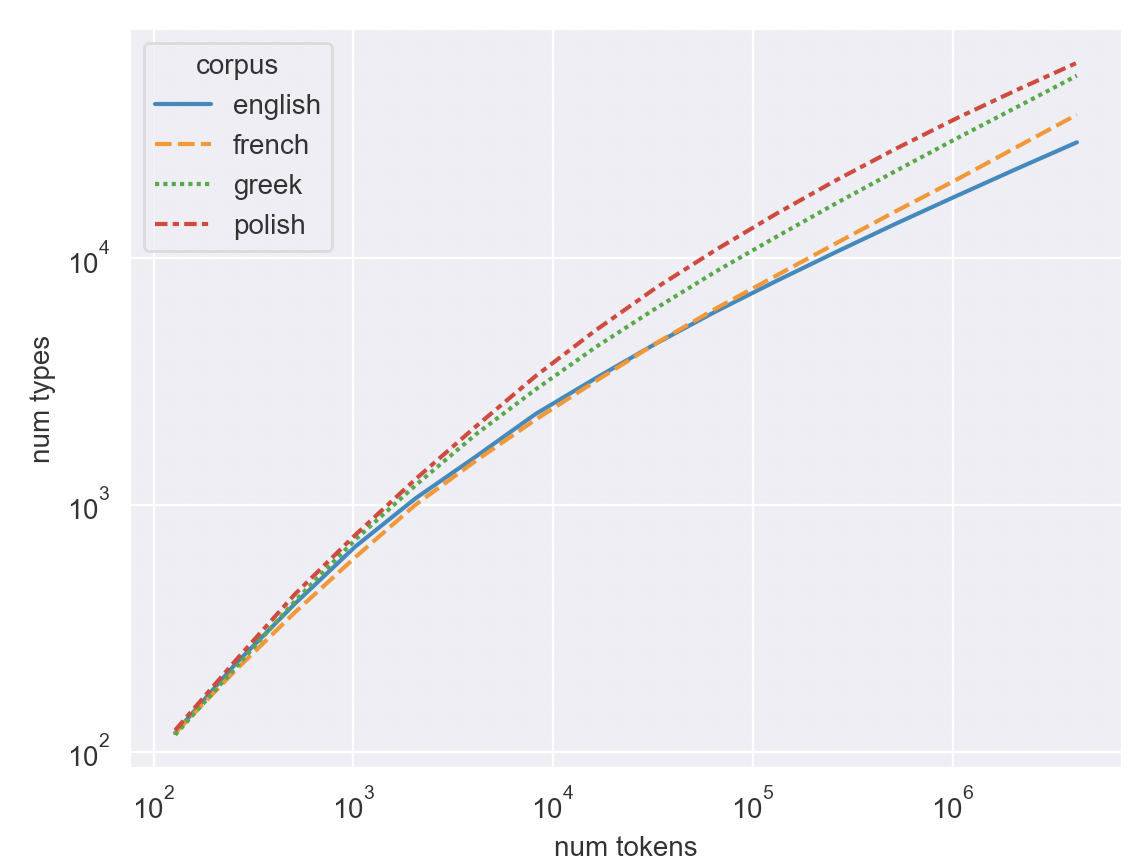
\includegraphics[width=0.48\textwidth]{images/type_token1.png}
\caption{Number of noun types versus number of observed noun tokens in the Europarl corpus.}
\label{fig:type_token1}
\end{figure}

\begin{figure}[t]
\centering
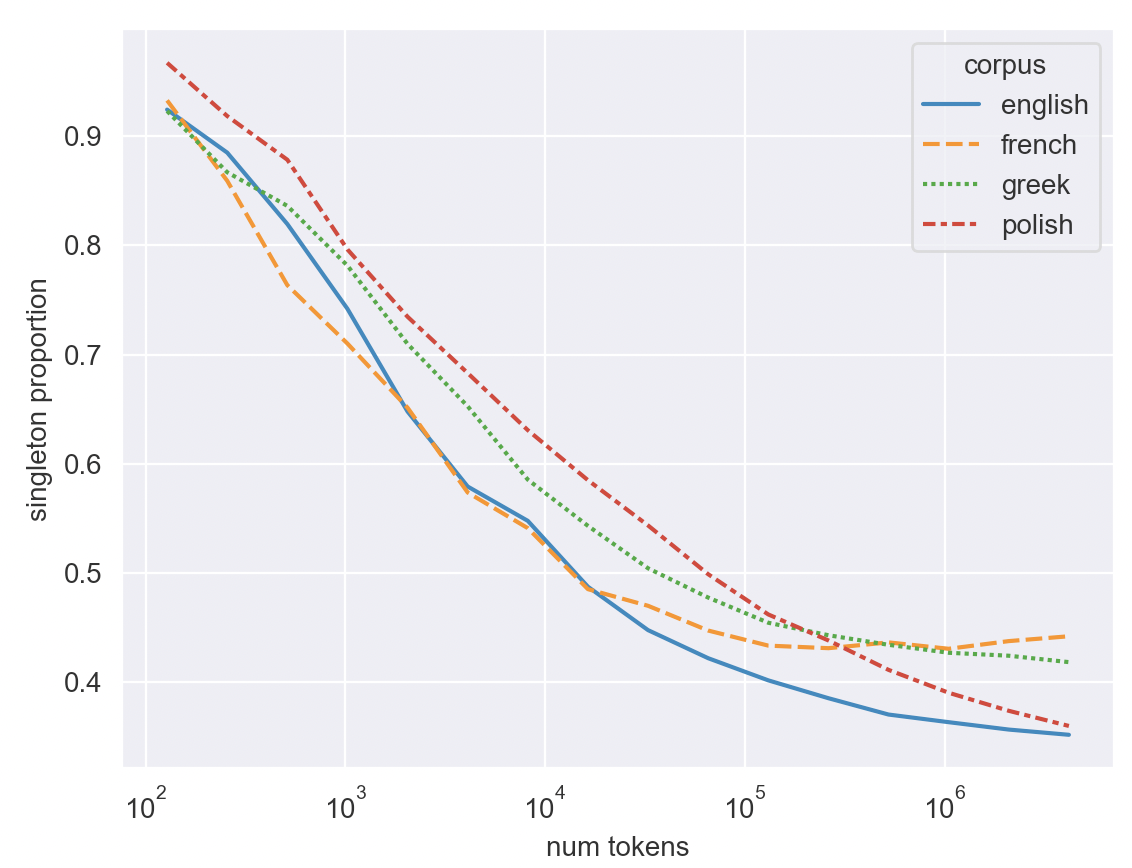
\includegraphics[width=0.48\textwidth]{images/sp1.png}
\caption{Singleton proportion versus number of observed noun tokens in the Europarl corpus.}
\label{fig:sp1}
\end{figure}

\subsection{Pitman-Yor Processes}

Let's begin by considering the noun distribution $\tau(\bnfpn{1})$. One strategy could be to collect a histogram of nouns from a corpus and normalize the histogram to create the distribution. But this commits us to a vocabulary size and token probabilities that are specific to the size of the corpus. This will be inappropriate for generating larger corpora, as nouns are an ``open class" of tokens whose frequencies follow a power law distribution. In Figure~\ref{fig:type_token1}, we plot the number of noun types (i.e. unique nouns) versus noun tokens for increasingly large subsets of the Europarl corpus \cite{koehn-2005-europarl}. Observe that the number of types never converges -- new nouns continue to be discovered, no matter how large the corpus grows\footnote{The languages with richer morphology, Polish and Greek, have a higher type-token ratio than more analytic languages like English and French, but the ``heavy tail'' phenomenon manifests regardless of the language's morphological properties.}. This ``heavy tail" property of natural language tokens has been documented by \cite{newman2005power} and \cite{teh-2006-hierarchical}, among others.

Another way to visualize this property \cite{teh-2006-hierarchical} is to plot the proportion of singleton tokens against the overall number of observed\footnote{To generate Figures~\ref{fig:type_token1} and \ref{fig:sp1}, we shuffled the Europarl sentences and extracted the nouns using \texttt{spaCy}. The shuffling smooths irregularities caused by topic shift.} tokens. Notice that the singleton proportion appears to converge to somewhere between 30\% and 50\% as the corpus size grows -- another indicator that in natural language, we continue to encounter new tokens, no matter how many tokens have already been observed.

To model this behavior, \cite{teh-2006-hierarchical} suggests using a generalization of the Dirichlet distribution \cite{kotz2004continuous} known as the Pitman-Yor process \cite{pitman1997two}. A Pitman-Yor process $\mathsf{PY}(d, \theta, G_0)$ is characterized by a \emph{discount} parameter $d \in [0,1)$, a \emph{strength} parameter $\theta \in (-d,\infty)$, and a \emph{base distribution} $G_0$ over integers $\{1, ..., |W|\}$. We follow \cite{teh-2006-hierarchical} in describing a Pitman-Yor process as a stochastic process that generates samples $\langle x_1, x_2, ... \rangle$ from i.i.d. samples $\langle y_1, y_2, ... \rangle$ drawn from base distribution $G_0$. Intuitively, it is a ``rich-get-richer" process, in which the $j$th sample $x_j$ is set to either the value $y_i$ assigned to a previous $x$-sample (with probability proportional to the number of previous $x$-samples that were assigned the value $y_i$), or the next $y$-sample in the sequence that hasn't yet been used. Formally, let $b_1=1$ and draw subsequent binary values $b_{n+1}$ from a Bernoulli (coin-flip) distribution where:
\begin{equation*}
	P(b_{n+1} = 1) =\frac{\theta + d\sum\limits_{1 \leq i \leq n} b_i}{\theta + n} 
\end{equation*}

\noindent Now define $t_1 = 1$ and consider $j, n \in \mathbb{Z}^+$. If $b_{n+1}=0$, then let $t_{n+1}=j$ with probability:
\begin{equation*}
	\frac{1}{n} \sum\limits_{1 \leq i \leq n} \mathbbm{1}(t_i=j)
\end{equation*}
Otherwise, if $b_{n+1}=1$: 
\begin{equation*}
t_{n+1}=1 + \sum\limits_{1 \leq i \leq n} b_i
\end{equation*}

\noindent The $n$th sample drawn from the Pitman-Yor process is $x_n = y_{t_n}$.

A Pitman-Yor process, for all practical purposes, can generate an "open-class" of words by using a uniform base distribution $G_0$ with a sufficiently large vocabulary size $|W|$ (for our experiments, we use the space of all 32-bit integers). However, we still need to choose appropriate discount and strength parameters.

\begin{figure}[t]
\centering
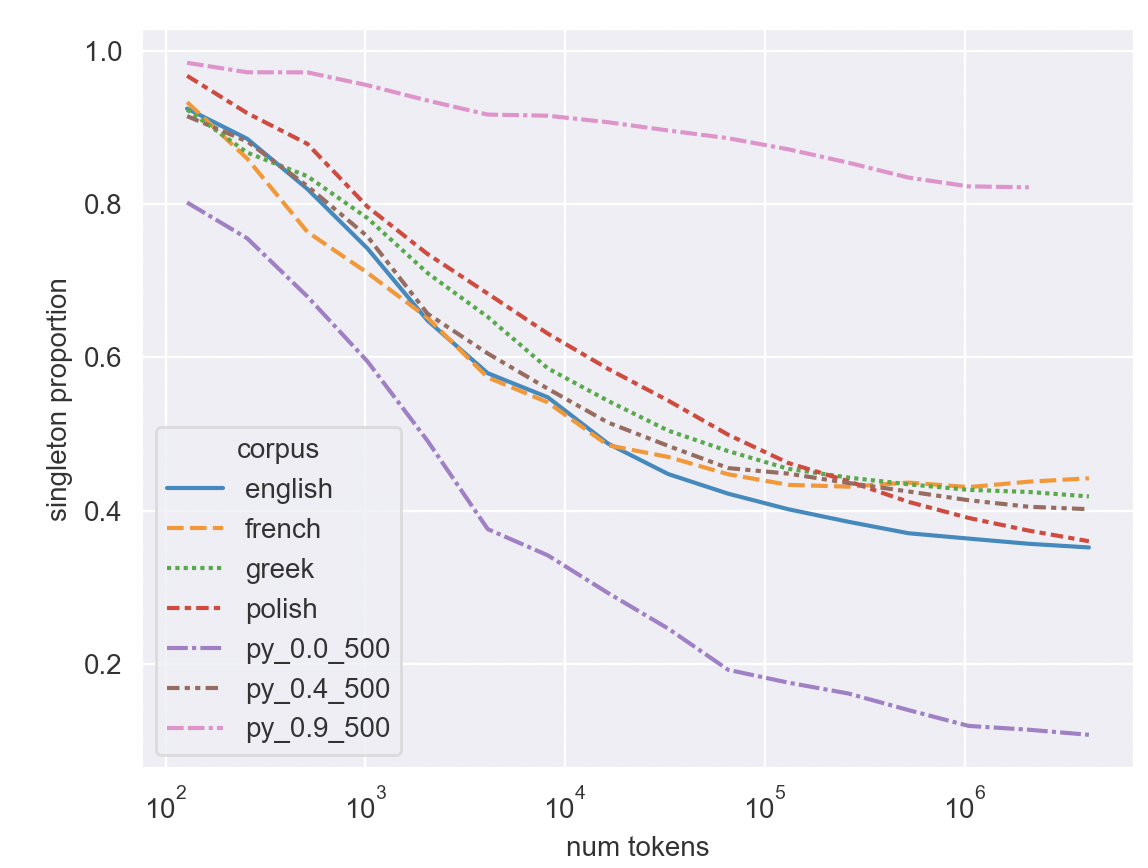
\includegraphics[width=0.48\textwidth]{images/sp2.png}
\caption{A comparison of the singleton proportion curves generated by Pitman-Yor processes with the curves of observed noun tokens in the Europarl corpus.}
\label{fig:sp2}
\end{figure}

\begin{figure}[t]
\centering
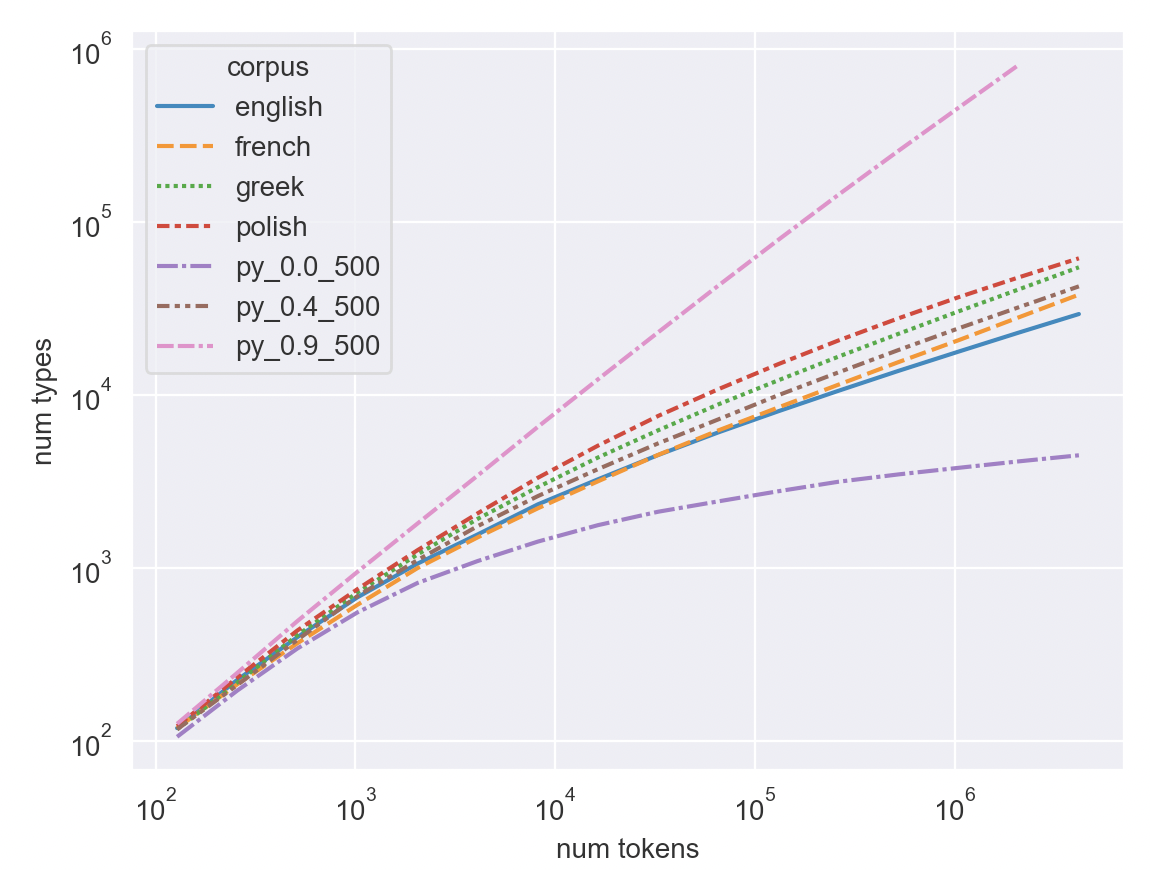
\includegraphics[width=0.48\textwidth]{images/type_token2.png}
\caption{A comparison of the type-token ratio curves generated by Pitman-Yor processes with the curves of observed noun tokens in the Europarl corpus.}
\label{fig:type_token2}
\end{figure}


In Figure~\ref{fig:sp2}, we plot the singleton proportion curves of tokens generated by various Pitman-Yor processes, and compare them with the singleton proportion curves of Europarl nouns. We find that $\mathsf{PY}(0.4, 500, G_0)$ closely follows the natural language curves. We obtain a similar correspondence when we plot the number of types versus the number of tokens (Figure~\ref{fig:type_token2}).


\subsection{Hierarchical Pitman-Yor Processes}

A similar experiment shows that $\mathsf{PY}(0.4, 500, G_0)$ also closely mirrors the natural language statistics of adjectives across the selected Europarl languages. So what happens if we use the distribution $\mathsf{PY}(0.4, 500, G_0)$ for both the noun distribution (i.e. distribution $\bnfpn{1}$) and every adjective distribution $\bnfpn{2.y_1}$) of the weighted grammar macro in Figure~\ref{fig:gmacro2}? In other words, what if we ignore selectional preference and just create adjective distributions that are independent of the head noun?

\begin{figure}[t]
\centering
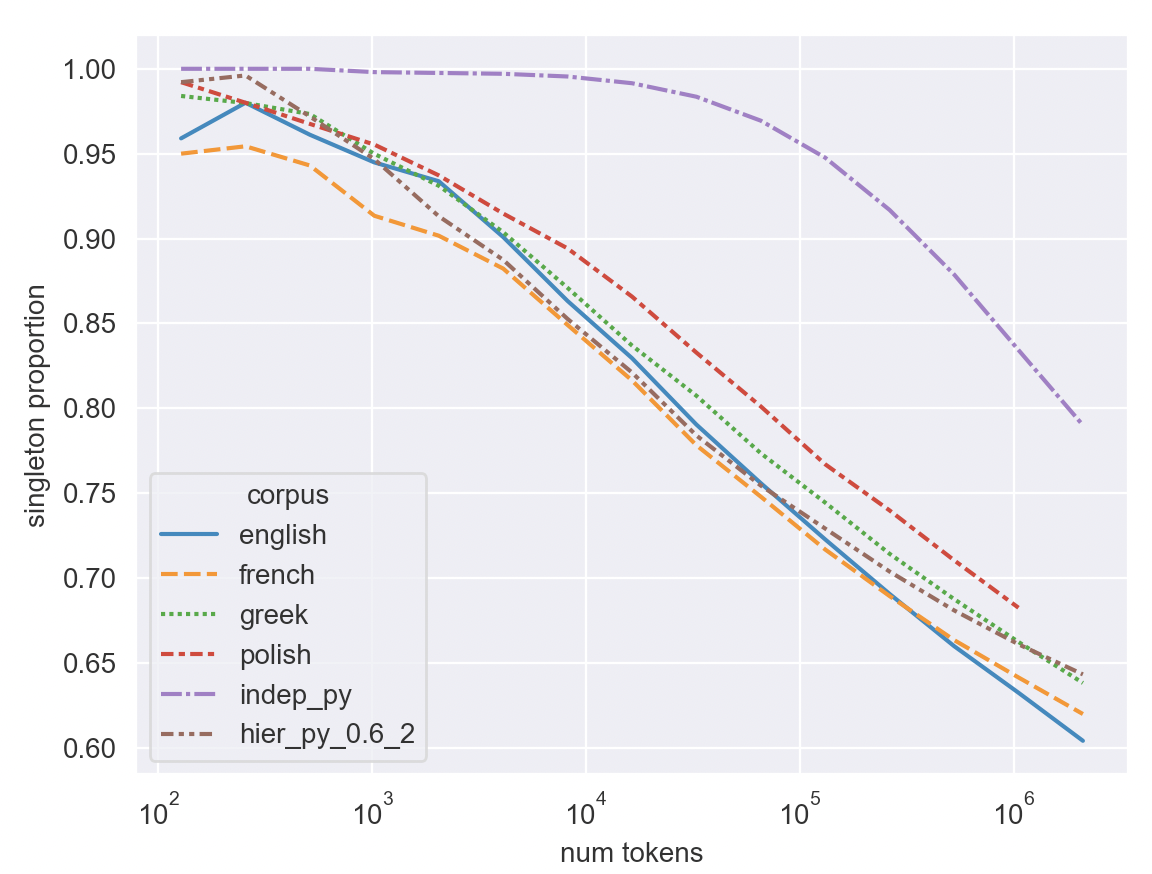
\includegraphics[width=0.48\textwidth]{images/sp3.png}
\caption{A comparison of the singleton proportion curves of adjective-noun bigrams in the Europarl corpus with bigrams generated from the macro in Figure~\ref{fig:gmacro2} using independent and hierarchical Pitman-Yor processes.}
\label{fig:sp3}
\end{figure}


To see what happens, we extract the adjective-noun bigrams from Europarl\footnote{We used \texttt{spaCy} to obtain universal dependency parses \cite{de-marneffe-etal-2014-universal} of the sentences, then extracted adjective-noun pairs related by the $\texttt{amod}$ dependency.} and plot singleton proportion curves of these extracted bigrams in Figure~\ref{fig:sp3}. The adjective-noun bigrams generated from independent distributions bear little resemblance to the natural language curves, confirming the importance of generating the adjectives from a noun-dependent distribution. To do so, we make use of a \emph{hierarchical Pitman-Yor process} \cite{teh-2006-hierarchical}.

A hierarchical Pitman-Yor process is simply a Pitman-Yor process that uses another Pitman-Yor process as its base distribution. For instance, we can define a global adjective distribution $G_\mathsf{2} = \mathsf{PY}(0.4, 500, G_0)$, and then for each noun $\bnfts{noun}.\bnfpn{y_1}$, we define a noun-dependent adjective distribution $G_\mathsf{\bnfpn{2.y_1}} = \mathsf{PY}(d, \theta, G_\bnfpn{2})$. Figure~\ref{fig:sp3} shows that using discount $d=0.6$ and strength $\theta=2$ (with base distribution $\mathsf{PY}(0.4, 500, G_0)$) provides a close match to the singleton proportion curves of natural language. The type-token ratio curves (omitted for space) tell the same story. 

\section{Experiments}

\begin{figure*}[p]
\centering
\begin{tabular}{rcl|l|l|l} 
&&&$w_\theta$&$w_\zeta$&switch\\
\hline \hline
$\bnfpn{S}$ &$\bnfpo$& $\bnfpn{S.z_1.z_2}$ & 1.0 & $\bnfpn{z_1} \mapsto \bnfpn{1}, \bnfpn{z_2} \mapsto \bnfpn{5}$ \\
$\bnfpn{S.y_1.y_2}$ &$\bnfpo$& $\bnfpn{NP.z_1.y_2} \bnfsp \bnfpn{VP.y_1.y_2}$ & 1.0 & $\bnfpn{z_1} \mapsto \bnfpn{2.1.y_1}$&1\\
$\bnfpn{NP.y_1.y_2}$ &$\bnfpo$& $\bnfpn{NPB.y_1.y_2} $ & 0.33 & \\
$\bnfpn{NP.y_1.y_2}$ &$\bnfpo$& $\bnfpn{NPB.y_1.y_2} \bnfsp \bnfpn{PP.z_1}$ & 0.33 & $\bnfpn{z_1} \mapsto \bnfpn{2.3.y_1}$ & 4\\
$\bnfpn{NP.y_1.y_2}$ &$\bnfpo$& $\bnfpn{NPB.y_1.y_2} \bnfsp \bnfpn{REL.z_1.y_2}$ & 0.33 & $\bnfpn{z_1} \mapsto \bnfpn{1.y_1}$ & 6\\
$\bnfpn{NPB.y_1.y_2}$ &$\bnfpo$& $\bnfpn{DT.y_2} \bnfsp \bnfpn{NN.y_1.y_2}$ & 0.5 & \\
$\bnfpn{NPB.y_1.y_2}$ &$\bnfpo$& $\bnfpn{DT.y_2} \bnfsp \bnfpn{ADJ.z_1} \bnfsp \bnfpn{NN.y_1.y_2}$ & 0.5 & $\bnfpn{z_1} \mapsto \bnfpn{3.y_1}$ & 5\\
$\bnfpn{VP.y_1.y_2}$ &$\bnfpo$& $\bnfpn{VB.y_1.y_2} \bnfsp \bnfpn{NP.z_1.z_2}$ & 0.5 & $\bnfpn{z_1} \mapsto \bnfpn{2.2.y_1}, \bnfpn{z_2} \mapsto \bnfpn{5}$ & 2\\
$\bnfpn{VP.y_1.y_2}$ &$\bnfpo$& $\bnfpn{VB.y_1.y_2} \bnfsp \bnfpn{COMP.z_1.z_2}$ & 0.5 & $\bnfpn{z_1} \mapsto \bnfpn{1}, \bnfpn{z_2} \mapsto \bnfpn{5}$ & 2\\
$\bnfpn{PP.y_1}$ &$\bnfpo$& $\bnfpn{PREP.z_1} \bnfsp \bnfpn{NPB.y_1.z_2}$ & 1.0 & $\bnfpn{z_1} \mapsto \bnfpn{4.y_1}, \bnfpn{z_2} \mapsto \bnfpn{5}$ & 4\\
$\bnfpn{REL.y_1.y_2}$ &$\bnfpo$& $\bnfts{who} \bnfsp \bnfpn{VP.y_1.y_2}$ & 1.0 & & 6 \\
$\bnfpn{COMP.y_1.y_2}$ &$\bnfpo$& $\bnfts{that} \bnfsp \bnfpn{S.y_1.y_2}$ & 1.0 & & 3\\
$\bnfpn{NN.y_1.y_2}$ &$\bnfpo$& $\bnfts{noun}.\bnfpn{y_1.y_2}$ & 1.0 & \\
$\bnfpn{VB.y_1.y_2}$ &$\bnfpo$& $\bnfts{verb}.\bnfpn{y_1.y_2}$ & 1.0 & \\
$\bnfpn{ADJ.y_1}$ &$\bnfpo$& $\bnfts{adj}.\bnfpn{y_1}$ & 1.0 & \\
$\bnfpn{DT.y_1}$ &$\bnfpo$& $\bnfts{dt.def}.\bnfpn{y_1}$ & 0.5 & \\
$\bnfpn{DT.y_1}$ &$\bnfpo$& $\bnfts{dt.indef}.\bnfpn{y_1}$ & 0.5 & \\
$\bnfpn{PREP.y_1}$ &$\bnfpo$& $\bnfts{prep}.\bnfpn{y_1}$ & 1.0 & \\
\end{tabular}
\caption{A weighted grammar macro that produces simple declarative sentences. As in \citet{white-cotterell-2021-examining}, certain rule macros are associated with ``switches.'' When the indicated switch is active, the RHS symbols are reversed if there are only two of them. The ``switched'' version of macro $\bnfpn{NPB.y_1.y_2} \bnfpo \bnfpn{DT.y_2} \bnfsp \bnfpn{ADJ.z_1} \bnfsp \bnfpn{NN.y_1.y_2}$ is $\bnfpn{NPB.y_1.y_2} \bnfpo \bnfpn{DT.y_2}  \bnfsp \bnfpn{NN.y_1.y_2} \bnfsp \bnfpn{ADJ.z_1}$. \label{fig:white1}}
\end{figure*}

\begin{figure*}[p]
\centering
\begin{tabular}{lll} 
$c$&$\tau(c)$&description\\
\hline \hline
$\bnfpn{1}$ & $\mathsf{PY}(0.4, 500, G_0)$ & global verb distribution \\
$\bnfpn{1.y_1}$ & $\mathsf{PY}(0.6, 20, \tau(\bnfpn{1}))$ & noun-dependent verb distribution \\
&& (for determining the head verb of relative clauses) \\
$\bnfpn{2}$ & $\mathsf{PY}(0.4, 500, G_0)$ & global noun distribution \\
$\bnfpn{2.1}$ & $\mathsf{PY}(0.4, 500, \tau(\bnfpn{2}))$ & global subject distribution \\
$\bnfpn{2.1.y_1}$ & $\mathsf{PY}(0.6, 20, \tau(\bnfpn{2.1}))$ & subject distribution for head verb $\bnfpn{y_1}$ \\
$\bnfpn{2.2}$ & $\mathsf{PY}(0.4, 500, \tau(\bnfpn{2}))$ & global object distribution \\
$\bnfpn{2.2.y_1}$ & $\mathsf{PY}(0.6, 20, \tau(\bnfpn{2.2}))$ & object distribution for head verb $\bnfpn{y_1}$ \\
$\bnfpn{2.3}$ & $\mathsf{PY}(0.4, 500, \tau(\bnfpn{2}))$ & global prepositional object distribution \\
$\bnfpn{2.3.y_1}$ & $\mathsf{PY}(0.6, 20, \tau(\bnfpn{2.3}))$ & prepositional object distribution for head noun $\bnfpn{y_1}$ \\
$\bnfpn{3}$ & $\mathsf{PY}(0.4, 500, G_0)$ & global adjective distribution \\
$\bnfpn{3.y_1}$ & $\mathsf{PY}(0.6, 2, \tau(\bnfpn{3}))$ & adjective distribution for head noun $\bnfpn{y_1}$\\
$\bnfpn{4}$ & $\mathsf{Unif}(\{1, ..., 20\})$ & global preposition distribution \\
$\bnfpn{4.y_1}$ & $\mathsf{PY}(0, 10, \tau(\bnfpn{4}))$ & preposition distribution for head noun $\bnfpn{y_1}$\\
$\bnfpn{5}$ & $\mathsf{Unif}(\{1, 2\})$ & global count distribution (1=singular, 2=plural) \\
\end{tabular}
\caption{Weighting table for Figure~\ref{fig:white1}. $G_0$ is a uniform distribution over all 32-bit integers. \label{fig:white2}}
\end{figure*}

\begin{figure*}[p]
\centering
\begin{tabular}{lll} 
Leefritish flobs who lalikize the flalocish bugogul along the flimik dakize these dumigs.\\
Flobs from huls dakize a lug to a flim.\\
A chulish flob jojotizes these cofapish moods at these chucish mooflofs.\\
The glofril beneath the mooduchogunish mob bapizes that the leefritish flob frichakupizes gluchols.\\
The leefritish chut beneath these dofils keemizes the kilirish jikoflog by a frukiloxish bomeegop.\\
A flob before the betish guf dakizes these moojatish chuflafs.
\end{tabular}
\caption{Selected sentences from a corpus generated using the weighted grammar macro defined by Figures~\ref{fig:white1} and \ref{fig:white2}, showcasing sentences that use the verb $\bnfts{dakize}$, the noun $\bnfts{flob}$, and the adjective $\bnfts{leefritish}$. \label{fig:white3}}
\end{figure*}


As a pilot study of our framework, we re-created an experiment performed by \citet{white-cotterell-2021-examining}, who used WCFGs to investigate the inductive biases of neural language models for various word orders exhibited by natural language. We created a weighted grammar macro (Figures~\ref{fig:white1} and \ref{fig:white2}) based on their WCFG description, which produces simple declarative sentences with relative clauses, prepositional phrases, and clausal complements. To extend their WCFG to accommodate selectional preference, we use the following compound nonterminals:

\begin{itemize}
	\item $\bnfpn{S.y_1.y_2}$: produces a sentence with subject count $\bnfpn{y_2}$ (if $\bnfpn{y_2}=1$, then the subject is singular; if $\bnfpn{y_2}=2$, then the subject is plural), whose head is the $\bnfpn{y_1}^{\mathsf{th}}$ verb of the vocabulary
	\item $\bnfpn{NP(B).y_1.y_2}$: produces a (base) noun phrase with count $\bnfpn{y_2}$, whose head is the $\bnfpn{y_1}^{\mathsf{th}}$ noun of the vocabulary
	\item $\bnfpn{VP.y_1.y_2}$: produces a verb phrase with subject count $\bnfpn{y_2}$, whose head is the $\bnfpn{y_1}^{\mathsf{th}}$ verb of the vocabulary
	\item $\bnfpn{PP.y_1}$: produces a prepositional phrase that modifies a noun phrase whose head is the $\bnfpn{y_1}^{\mathsf{th}}$ noun of the vocabulary
	\item $\bnfpn{REL.y_1.y_2}$: produces a relative clause with subject count $\bnfpn{y_2}$, whose head is the $\bnfpn{y_1}^{\mathsf{th}}$ verb of the vocabulary
	\item $\bnfpn{COMP.y_1.y_2}$: produces a clausal complement with subject count $\bnfpn{y_2}$, whose head is the $\bnfpn{y_1}^{\mathsf{th}}$ verb of the vocabulary
	\item $\bnfpn{NN.y_1.y_2}$: produces the $\bnfpn{y_1}^{\mathsf{th}}$ noun of the vocabulary, declined for count $\bnfpn{y_2}$
	\item $\bnfpn{VB.y_1.y_2}$: produces the $\bnfpn{y_1}^{\mathsf{th}}$ verb of the vocabulary, conjugated for subject count $\bnfpn{y_2}$
	\item $\bnfpn{ADJ.y_1}$: produces the $\bnfpn{y_1}^{\mathsf{th}}$ adjective of the vocabulary
	\item $\bnfpn{DET.y_1}$: produces a determiner for a noun with count $\bnfpn{y_1}$
	\item $\bnfpn{PREP.y_1}$: produces the $\bnfpn{y_1}^{\mathsf{th}}$ preposition of the vocabulary
\end{itemize}

We used a voicebox that assigned concatenations of random syllables to each generic noun, verb, and adjective. It used English prepositions, determiners, and morphology (e.g. verbs with a singular subject were suffixed with the letter ``s''). To enhance interpretability\footnote{This also likely made the language easier for the language models to learn.} for English speakers, the voicebox also added the suffix "-ize" to verbs and "-ish" to adjectives. Figure~\ref{fig:white3} presents a selection of sentences from a corpus generated by our grammar macro.

\begin{figure*}[t]
\centering
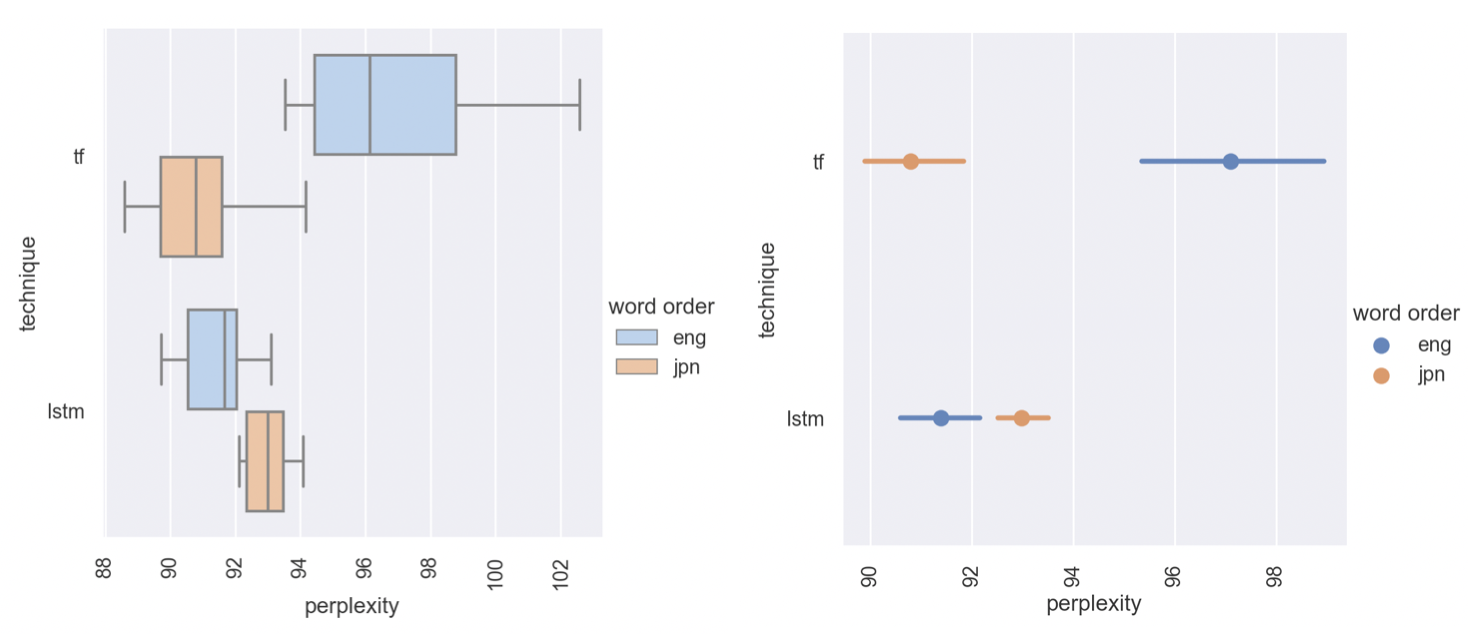
\includegraphics[width=.96\textwidth]{images/results.png}
\caption{Visualization of experimental results using a box plot (left) and point plot (right). The transformer produces lower-perplexity language models for the artificial languages that follow a Japanese word order, while the LSTM produces lower-perplexity language models for the artificial languages that follow an English word order.}
\label{fig:results}
\end{figure*}


We set the parameters of our Pitman-Yor processes (refer to Figure~\ref{fig:white2}) using the methodology described in Section~\ref{sec:powerlaw}, specifying discount and strength parameters so that our produced sentences closely matched the type-token ratio and singleton proportion curves of the English, French, Greek, and Polish Europarl corpora for the following n-grams:
\begin{enumerate}
	\item \textbf{unigrams}: nouns, verbs, adjectives
	\item \textbf{bigrams}: adjective-noun, verb-subject, verb-object
	\item \textbf{trigrams}: subject-verb-object 
\end{enumerate}
\noindent As in Section~\ref{sec:powerlaw}, these n-grams were extracted using \texttt{spaCy} universal dependency parsers and taggers.

Following \citet{white-cotterell-2021-examining}, we created $2^6=64$ variants of the grammar macro, corresponding to the possible configuration of six binary typological ``switches":
\begin{enumerate}
	\item \textbf{$\bnfpn{S}$-switch}: the position of the subject in a sentence, relative to the head verb 
	\item \textbf{$\bnfpn{VP}$-switch}: the position of the head verb in a verb phrase, relative to the object or complement
	\item \textbf{$\bnfpn{Comp}$-switch}: the position of the complementizer in a complement, relative to the sentential component
	\item \textbf{$\bnfpn{PP}$-switch}: the position of the preposition\footnote{Technically, these are \emph{adpositions}, since they can now appear before or after their objects.} in a prepositional phrase, relative to the prepositional object
	\item \textbf{$\bnfpn{NP}$-switch}: the position of the adjective in a noun phrase, relative to the head noun
	\item \textbf{$\bnfpn{Rel}$-switch}: the position of a relative clause, relative to the noun it modifies
\end{enumerate}
\noindent Figure~\ref{fig:white1} annotates the affected rule macros with their switches. When a switch was set to zero (i.e. the switch was ``off''), then the rule macro was used as-is. When a switch was set to one (i.e. the switch was ``on''), then an alternative version of the rule macro was used. In all but one case, the alternative just swaps the two RHS symbols; the one exception is the $\bnfpn{NP}$ switch, which replaces macro $\bnfpn{NPB.y_1.y_2} \bnfpo \bnfpn{DT.y_2} \bnfsp \bnfpn{ADJ.z_1} \bnfsp \bnfpn{NN.y_1.y_2}$ with macro $\bnfpn{NPB.y_1.y_2} \bnfpo \bnfpn{DT.y_2}  \bnfsp \bnfpn{NN.y_1.y_2} \bnfsp \bnfpn{ADJ.z_1}$. Switch configuration \texttt{000000} (all switches off) corresponds to a standard English word order, whereas switch configuration \texttt{011101} (i.e. switches 2, 3, 4, 6 are on) corresponds\footnote{\citet{white-cotterell-2021-examining} used \texttt{000000} to refer to Japanese word order. Since the interpretation of an ``on'' switch is arbitrary, we used \texttt{000000} to refer to English word order so that the default syntax of Figure~\ref{fig:white1} would be more familiar to English speakers.} to a standard Japanese word order.

Initially, again following \citet{white-cotterell-2021-examining}, we generated 100,000 sentences for each of the 64 grammar macro variants, and divided these into ten evenly sized corpora. Each corpus of 10,000 sentences was further divided into an 8000-1000-1000 train-dev-test partition. On each train set, we trained\footnote{Like \citet{white-cotterell-2021-examining}, we used the \texttt{fairseq} implementation \cite{ott-etal-2019-fairseq} of these language models.} a transformer-based and an LSTM-based language model, resulting in 10 language models per choice of neural architecture and switch configuration. Finally, we evaluated these LMs on the respective test sets. 


Unfortunately, with only 8000 training sentences per trial, we did not obtain statistically significant results\footnote{\citet{white-cotterell-2021-examining} did get statistically significant results using this experimental set-up, but likely this is attributable to a smaller vocabulary and less ``natural" token distributions.}. As our primary goal with this work was to introduce a theoretical framework, rather than to perform a specific empirical investigation, we proceeded with a narrower version of the \citet{white-cotterell-2021-examining} experiment. We focused on the two switch configurations (\texttt{000000} and \texttt{011101}) that correspond to the standard word orders of English and Japanese, and augmented the generation (for each trial) from 8k-1k-1k datasets to 800k-100k-100k datasets. 


For each architecture (transformer and LSTM) and word order (English and Japanese), Figure~\ref{fig:results} visualizes the test perplexity over the ten trials using two graphs: a box plot and a point plot\footnote{We used \texttt{seaborn} to generate the plots. For those unfamiliar, the box plot shows the median trial (vertical line inside the box), the 25th-75th percentile trials (the box) and the entire range of the trials (the ``whiskers"). The point plot shows the mean of the trials (the dot) and the 95\% confidence interval (the line).}. For transformer LMs, we obtained lower perplexity on the languages that followed a Japanese word order. For LSTM LMs, we observed the opposite: a (statistically significant) lower perplexity on the languages that followed an English word order.

These results generally support the findings of \citet{white-cotterell-2021-examining}, except that \citet{white-cotterell-2021-examining} did not find significant differences between any of their trained LSTM LMs -- indeed, our observed differences are not nearly as large as those observed between the transformer LMs. We find it encouraging that our results do not differ wildly from \citet{white-cotterell-2021-examining} (it would be troubling for the prospects of artificial languages if each iterative improvement dramatically reversed the conclusions of the previous iteration). At the same time, we also find it encouraging that the differences between their results and ours offer a possible reconciliation between \citet{white-cotterell-2021-examining} and \citet{ravfogel-etal-2019-studying}, who reported, based on experiments with naturally-derived corpora, that LSTM LMs performed better on SVO (versus SOV) languages.




\section{Conclusion}

With this work, our goal is to enable researchers to more easily develop models for typologically diverse languages, and to investigate under what conditions such models perform effectively. By demonstrating how weighted grammar macros can model realistic syntactic and semantic dependencies, we hope to provide some confidence that the framework can prove a useful substitute for real-world data, when such data is not readily available.

To facilitate adoption of our framework, we will accompany this paper with the release of an open-source Python package\footnote{The package is already prepared, unit tested, and documented.} for building weighted grammar macros, providing fellow researchers with a means to generate artificial languages that emulate the typology of the natural languages they seek to study. 


%\appendix

%\section{Additional Experimental Details}

%The experiments were run on a single workstation with the following specifications:
%\begin{itemize}
%	\item \textbf{Operating System:} Ubuntu 18.04 	
%	\item \textbf{Processor:} Intel Xeon E5-1650 v4 (6 core)
%	\item \textbf{GPUs:} 4x NVIDIA GeForce GTX 1080Ti
%	\item \textbf{Memory:} 128 GB DDR4 RAM
%\end{itemize}

%\noindent The language models were trained with the following command:

%\noindent
%\small
%\texttt{fairseq-train \\
%  --task language\_modeling \\
%  --arch \{transformer\_lm, lstm\_lm\} \
%  --share-decoder-input-output-embed \
%  --dropout 0.1 \
%  --optimizer adam \
%  --adam-betas '(0.9, 0.98)' \
%  --weight-decay 0.01 \\
%  --clip-norm 0.0 \
%  --lr 0.0005 \
%  --lr-scheduler inverse\_sqrt \
%  --warmup-updates 4000 \
%  --warmup-init-lr 1e-07 \
%  --tokens-per-sample 512 \
%  --sample-break-mode none \\
%  --max-tokens 2048 \
%  --update-freq 16 \
%  --patience 15 \
%  --fp16 \\
%  --max-update 50000}


\bibliography{anthology,custom}
\bibliographystyle{acl_natbib}

\appendix


\end{document}


